\documentclass[12pt,oneside]{article}
\usepackage{times,mathptmx}
\usepackage[pdftex]{graphicx}
\usepackage{calc}
\usepackage{tabularx,ragged2e,booktabs,caption,subcaption}
\usepackage{array}
\newcolumntype{L}[1]{>{\raggedright\let\newline\\\arraybackslash\hspace{0pt}}m{#1}}
\newcolumntype{C}[1]{>{\centering\let\newline\\\arraybackslash\hspace{0pt}}m{#1}}
\newcolumntype{R}[1]{>{\raggedleft\let\newline\\\arraybackslash\hspace{0pt}}m{#1}}
\usepackage{multirow}
\usepackage{tocloft}
\usepackage{xcolor}
\usepackage{color,soul}
\usepackage{amsmath}
\definecolor{linknavy}{rgb}{0,0,0.50196}
\definecolor{linkred}{rgb}{1,0,0}
\definecolor{linkblue}{rgb}{0,0,1}
\usepackage{float}
\usepackage{graphpap}
\usepackage{rotating}
\usepackage{graphicx}
\usepackage{geometry}
\usepackage{relsize}
\usepackage{ltablex}
\usepackage{longtable}
\usepackage{lscape}
\usepackage{amssymb}
\usepackage{makeidx} % Create index at end of document
\usepackage[nottoc,notlof,notlot]{tocbibind} % Put the bibliography and index in the ToC
\usepackage{lastpage} % Automatic last page number reference.
\usepackage[T1]{fontenc}
\usepackage{enumerate}
\usepackage{upquote}
\usepackage{moreverb}
\usepackage{xfrac}
\usepackage{cite}
\usepackage{tikz}
% \usepackage{subfig}
% \usepackage{caption}
\usepackage[toc,page]{appendix}
\usepackage{notoccite}

\usepackage{titlesec}
\titleformat{\chapter}[hang] 
{\normalfont\huge\bfseries}{\chaptertitlename\ \thechapter}{1em}{} 

\newcommand{\nopart}{\expandafter\def\csname Parent-1\endcsname{}} % To fix table of contents in pdf.

\usepackage{siunitx}
\sisetup{
    detect-all = true,
    input-decimal-markers = {.},
    input-ignore = {,},
    inter-unit-product = \ensuremath{{}\cdot{}},
    multi-part-units = repeat,
    number-unit-product = \text{~},
    per-mode = fraction,
    separate-uncertainty = true,
}

\usepackage{listings}
\usepackage{textcomp}
\definecolor{lbcolor}{rgb}{0.96,0.96,0.96}

\usepackage[pdftex,
        colorlinks=true,
        urlcolor=linkblue,     % \href{...}{...} external (URL)
        citecolor=linkred,     % citation number colors
        linkcolor=linknavy,    % \ref{...} and \pageref{...}
        pdfproducer={pdflatex},
        pdfpagemode=UseNone,
        bookmarksopen=true,
        plainpages=false,
        verbose]{hyperref}

\setlength{\textwidth}{6.5in}
\setlength{\textheight}{9.0in}
\setlength{\topmargin}{0.in}
\setlength{\headheight}{0.pt}
\setlength{\headsep}{0.in}
\setlength{\parindent}{0.0in}
\setlength{\itemindent}{0.25in}
\setlength{\oddsidemargin}{0.0in}
\setlength{\evensidemargin}{0.0in}
% \setlength{\leftmargini}{\parindent} % Controls the indenting of the "bullets" in a list
\setlength{\cftsecnumwidth}{0.45in}
\setlength{\cftsubsecnumwidth}{0.5in}
\setlength{\cftfignumwidth}{0.45in}
\setlength{\cfttabnumwidth}{0.45in}
\setlength{\parskip}{1em}

\newcommand{\titlesigs}
{
\large
\flushright{UL Firefighter Safety Research Institute\\
{\em Stephen Kerber, Director} \\
\hspace{1in} \\
}
}

\newcommand{\headerB}[1]{
\flushleft{
\fontsize{28}{33.6}\selectfont
\bf{#1}
}
}

\newcommand{\headerC}[1]{
\vspace{.5in}
\flushright{\fontsize{14}{16.8}\selectfont
#1}
}

% \newcolumntype{L}{>{\centering\arraybackslash}m{4cm}}

\floatstyle{boxed}
\newfloat{notebox}{H}{lon}
\newfloat{warning}{H}{low}

\newenvironment{conditions}
  {\par\vspace{\abovedisplayskip}\noindent\begin{tabular}{>{$}l<{$} @{${}={}$} l}}
  {\end{tabular}\par\vspace{\belowdisplayskip}}


% Rename chapter headings
% \renewcommand{\chaptername}{}
% \renewcommand{\bibname}{References}

\usepackage{fancyhdr}
\usepackage{placeins}
\pagestyle{fancy}
\lhead{}
\rhead{}
\chead{}
\renewcommand{\headrulewidth}{0pt}

% UN-COMMENT TO PLACE WATERMARK
\usepackage{draftwatermark}
\SetWatermarkText{DRAFT}
\SetWatermarkScale{1}

\usepackage{subcaption}
\usepackage{xfrac}

\begin{document}

% \frontmatter

\begin{center}
\large{Residential Structure Fire Intervention and Victim Tenability}\\
\normalsize{$^1$Steve Kerber, $^2$Gavin P. Horn, $^3$Kenneth W Fent, $^{2,4}$Denise L Smith, $^1$John Regan \\}
\end{center}

\flushright{$^1$ UL Firefighter Safety Research Institute; Columbia, MD, USA \\
$^2$ University of Illinois, Fire Service Institute; Urbana-Champaign, IL, USA\\
$^3$ National Institute for Occupational Safety \& Health; Cincinnati, OH, USA \\
$^4$ Skidmore College; Saratoga Springs, NY }

\vspace{2in}

\flushleft{Address correspondence to:\\
Steve Kerber\\
UL Firefighter Safety Research Institute \\
6200 Old Dobbin Lane, Suite 150\\
Columbia, MD 21045\\
USA\\

Telephone: 847.664.6999\\
E-mail: stephen.kerber@ul.com}
	
\vspace{1.5in}


\flushleft{Acknowledgements/Funding: This work was supported by the Department of Homeland Security Fire Prevention and Safety Grant \#EMW-2013-FP-00766. \\

Disclosure: There are no conflicts of interest regarding this work.}




\vfill

% \flushright{\includegraphics[width=2.in]{../8_Images/FSRI_GraphicShield}}

\titlesigs
\newpage
\section{Abstract}
% \mainmatter
\flushleft
\section{Introduction}
\label{sec:intro}

A primary goal of firefighting is to extinguish the fire to protect life and property. While this basic goal may seem obvious and straightforward to a civilian, the tactics used by the fire department to accomplish this goal may vary considerably. Based on an accumulating body of evidence, many fire departments are emphasizing applying water to the fire as soon as possible to improve conditions inside the structure (Kerber, 2013). Such an approach is often called a ``transitional'' attack in which firefighters apply water through a window to initially suppress the fire before they enter the building to completely extinguish the fire and ensure there is no further fire growth.  This approach contrasts with the approach that many departments that have been taught, which is that it is best to enter the house through the front door with a charged hose line. In theory, the goal of this ``interior'' fire attack is to find the seat of the fire and extinguish it as soon as possible to protect potential victims. To date, there is no research that has considered the effect of different firefighting tactics on the firefighter's physiological responses to their work and the impact on potential occupant survivability.

This paper will focus on occupant survivability and the interaction between firefighter suppression (transitional attack and direct interior attack) and search and rescue tactics on occupant survivability.  This will be done by utilizing building temperature and gas concentration measurements that were placed close to two simulated occupants.  

\section{Methods}
\label{sec:methods}

\subsection{Subjects}
Participants were recruited through a nationwide multimedia effort, along with a focused effort by a statewide network of firefighters who teach and train at the Illinois Fire Service Institute's (IFSI) Champaign campus. Forty (n=40) firefighters (36 male, 4 female) from departments in Illinois, Georgia, Indiana, Ohio, South Dakota and Wisconsin participated in this study. The firefighters were 37.6$\pm$8.9 years old, 1.80$\pm$0.08 m tall, weighed 89.8$\pm$14.5 kg and had an average BMI of 27.6$\pm$3.4 kg/m$^2$.

All participants were required to have completed a medical evaluation consistent with National Fire Protection Association (NFPA) 1582 in the past 12 months.An emphasis was placed on recruiting  experienced firefighters who had up to date training, could complete the assigned tasks as directed, and were familiar with live-fire policies and procedures. Throughout the study protocol, all firefighters were required to wear their self-contained breathing apparatus (SCBA) prior to entering the structure. The research team supplied all personal protective equipment (PPE) for the participants to enhance standardization and to ensure that all protective equipment adhered to NFPA standards.

\subsection{Study Design}

% The structure contained two six bedrooms, an open living/dining room, and a kitchen. The house was constructed so that the two bedrooms on the sides of the house could be sealed off from the rest of the structure, to facilitate turnover of the house between experiments. Thus, for each experiment, the structure contained two bedrooms that were open to the rest of the structure, two with closed doors, a kitchen, a living room, and a dining room. The layout for the two sides of the structure is shown in Figure \ref{fig:layout}. The fires were ignited  first in 

% \begin{figure}[!ht]
% 	\centering
% 	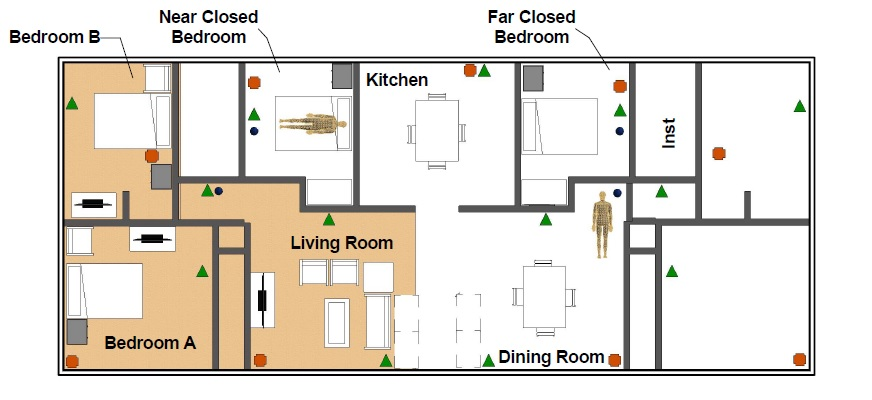
\includegraphics[width=.75\textwidth]{../Images/Left}
% 	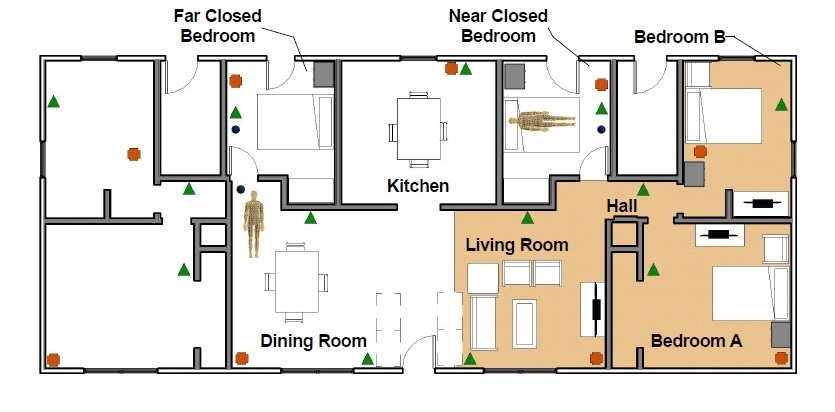
\includegraphics[width=.75\textwidth]{../Images/Right}
% 	\caption[Structure Layout and Instrument Locations]{Instrument Locations for Left (top) and Right (bottom) layouts}
% 	\label{fig:layout}
% \end{figure}
Teams of 12 firefighters were deployed to suppress fires in a realistic firefighting scenario that involved a multiple-room fire (two separate bedrooms) in a 111 m$^2$ residential structure. Each team of 12 firefighters worked in pairs to perform six different job assignments that included operations on the inside of the structure during active fire (fire attack and search \& rescue), on the outside of the structure during active fire (command \& pump operator and outside ventilation), and to conduct overhaul operations after the fire had been suppressed (firefighters searched for smoldering items and removed items from the structure).  
%The job assignments are described in Table . 

In all, 12 different trials were conducted (one per day) each with twelve firefighters as described above.  The firefighters responded to two scenarios that differed only in the tactics used by the Inside Attack team: (a) traditional interior attack from the ``unburned side'' (advancement through the front door to extinguish the fire) and (b) transitional attack (water applied into the bedroom fires through an exterior window - from the ``unburned side'' - prior to advancing through the front door to extinguish the fire).  The firefighters performed the same role using both tactics, then were reassigned to different job assignments and performed another two scenarios – again using the same two tactics on separate days.  While most firefighters attended four sessions of the study (n=31), a small group were only available for two sessions (n=9) and one firefighter withdrew from the study and wasn't replaced until after the first two scenarios.

\subsection{Study Protocol}
Following recruitment, subjects completed all required paperwork and anthropomorphic measurements (height, weight) were collected.  Firefighters received a core temperature pill that they ingested 6–12 hours prior to data collection. Upon arrival on each day, firefighters were instrumented with skin temperature patches on the back of their neck and upper arm that they wore throughout the trial. Multiple pre- and post-firefighting cardiovascular measurements and chemical exposure samples (biological and PPE) were collected prior to the initiation of the live fire evaluation (these data will be reported elsewhere).  The firefighter subjects were then deployed to complete their firefighting work in a purpose-built live-fire research test structure. 

In order to safely and reliably conduct this study, a structure was designed and built to have all of the interior finishes and features of a single family dwelling, yet contained specialized safety systems and hardened construction techniques that ensured participants' safety. The house was based on a design by a residential architectural company to be representative of a home constructed in the mid-twentieth century with walls and doorways separating all of the rooms and 2.4 m ceilings. The home had an approximate floor area of 111 m$^2$, with 8 total rooms, including 4 bedrooms and 1 bathroom (closed off during experiments). Interior finishes in the burn rooms were protected by 15.9 mm Type X gypsum board on the ceiling and 12.7 mm gypsum board on the walls. To maximize the use of the structure and minimize time between experiments, the house was mirrored so that there were 2 bedrooms on each side where the fires were ignited.  During each experiment a temporary wall was constructed at the end of the hallway to isolate 2 bedrooms so that they could be repaired and readied for the next experiment. The left and right layouts are shown in Figure \ref{fig:layout}.
\begin{figure}[!ht]
	\centering
	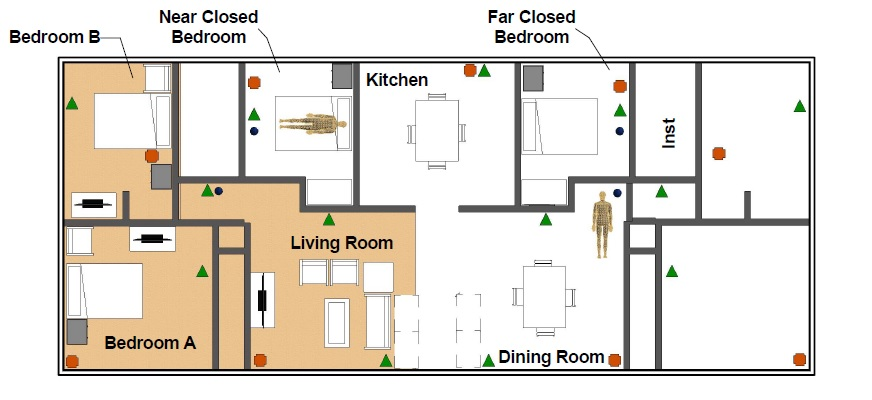
\includegraphics[width=.75\textwidth]{../Images/Left}
	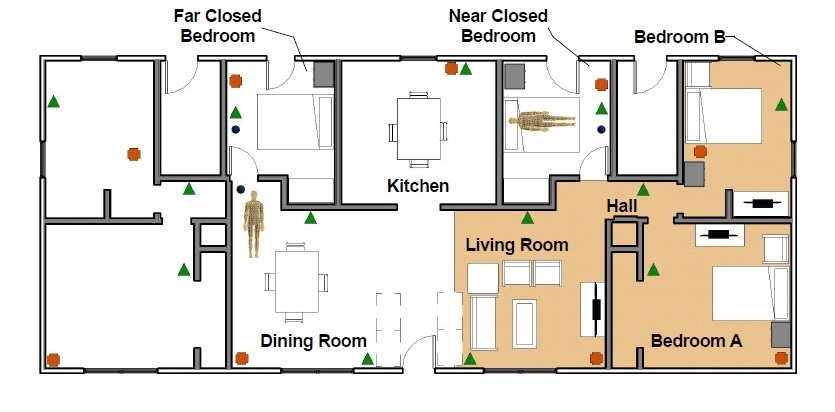
\includegraphics[width=.75\textwidth]{../Images/Right}
	\caption[Structure Layout and Instrument Locations]{Instrument Locations for Left (top) and Right (bottom) layouts}
	\label{fig:layout}
\end{figure}
Furniture was acquired from a single source such that each room was furnished identically (same item, manufacture, make model and layout of all furnishings) for all 12 experiments. The bedrooms, where the fires were ignited, were furnished with a double bed (covered with a foam mattress topper, comforter and pillow), stuffed chair, side table, lamp, dresser and flat screen television.  The floors were covered with polyurethane foam padding and polyester carpet.  All other rooms of the structure were also furnished to provide obstacles for the firefighter, but those furnishings were not involved in the fire. Figure 1 provides a rendering of the structure with the roof cut away to show the interior layout with furniture and floor coverings.  The tan floor shows the carpet placement and the gray floor shows the cement floor or simulated tile locations.  

Fires were ignited in the stuffed chair in Bedrooms  A and B using a remote ignition device and a book of matches to create a small flaming ignition source.  The flaming fire was allowed to grow until temperatures in the fire rooms reached levels determined to be near peak values based on pilot studies (i.e. room had ‘flashed over').  When interior temperatures of both fire rooms exceeded 600 $^{\circ}$C at the ceiling, the fire department dispatch was simulated and firefighters responded by walking approximately 16 meters from the data collection bay to the front of the structure.  The time of dispatch was between 4 and 5 minutes after ignition for all 12 experiments.  

\subsection{Measures}

\subsubsection{Building Temperature Measurements}
To assess fire dynamics throughout the fire scenarios, measurements included gas temperature, gas concentrations, pressure, heat flux, thermal imaging, and video recording. Detailed measurement locations can be found in Figure 1.  
Gas temperature was measured with bare-bead, ChromelAlumel (type K) thermocouples with a 0.5 mm nominal diameter. Thermocouple arrays were located in every room. The thermocouple locations in the living room, dining room, hallway, Bedroom 4, and kitchen had an array of thermocouples with measurement locations of 0.3 m, 0.6 m, 0.9 m, 1.2 m, 1.5 m, 1.8 m and 2.1 m above the floor. The thermocouple locations in Bedroom A and Bedroom B had an array of thermocouples with measurement locations of 0.3 m, 0.9 m, 1.5 m, and 2.1 m above the floor. 

\subsubsection{Building Gas Concentration Measurements}
Gas concentrations of oxygen, carbon monoxide, and carbon dioxide were measured (OxyMat 6 and Ultramat 23 NDIR; Siemens) at 0.9 m from the floor inside and outside of the closed bedrooms.   These measurement locations are adjacent to the simulated occupant sitting outside of the far bedroom and the simulated occupant laying on the bed in the near bedroom.  This measurement location is also consistent with a potential occupant crawling to escape the fire.  The uncertainty of the measured concentration is 1\% of the maximum concentration measurement. The maximum concentration measurements were 5\% for CO and 20\% for CO2. The gases were extracted from the corners of rooms so as to minimize risk of damage from removing burned fuels and touring visitors. All data was collected at a frequency of 1 Hz. 

\subsubsection{Firefighter Intervention Measurements}
For each scenario, firefighter intervention was monitored and recorded utilizing standard video cameras placed outside and throughout the structure.  Thermal imaging cameras were also placed inside the structure to examine firefighter movements and simulated occupant search and rescue tactics.  Portable cameras were also affixed to the simulated occupants to qualitatively capture their exposure and movements from their locations to the outside of the structure as the firefighters rescued them.

\subsection{Occupant Tenability}
Occupant tenability, which is the survivability of occupants in the fire environment, is a primary concern for any firefighting operation.  Two standard measures of occupant tenability were used during these experiments - temperature and gas concentration - based upon the fractional effective dose methodology (FED) from ISO 13571 []. This methodology provides a method to calculate the time to incapacitation based on an accumulated exposure to either toxic gases:
\begin{equation}\label{eqn:FED_co}FED_{CO} = \Sigma [\frac{\phi_{CO}}{3.5}*\nu_{CO_2}*\Delta t]\end{equation}

\begin{equation}\label{eqn:FED_vco2}\nu_{CO_2}=exp(\frac{\phi_{CO_2}}{5})\end{equation}
Or local ambient air temperature 

\begin{equation}\label{eqn:FED_temp}FED_{temp}=\Sigma[\frac{T^{3.61}}{4.1*10^8}*\Delta t]\end{equation}

where $\nu_{CO_2}$ is a frequency factor to account for the increased rate of breathing due to carbon dioxide, $\phi_{CO_2}$ and $\phi_{CO}$ are the mole fractions (\%) of carbon dioxide and carbon monoxide, T is the temperature near the occupant ($^{\circ}$C), and $\Delta$t is the time increment of the measurements made in the experiments in minutes (1/60 in these experiments).  According to ISO 13571, the uncertainty in Eq. 1 is $\pm$ 20\% and the uncertainty in Eq. 2 is $\pm$ 35\%.  Equation 3 only applies for temperatures greater than 120$^{\circ}$C, which is taken as the lower limit to this method. FED relates to the probability of the conditions being non-tenable for a certain percent of the population through a lognormal distribution.  For reference, FED = 0.3 is the criterion used to determine the time of incapacitation for susceptible individuals (young children, elderly, and/or unhealthy occupants) and corresponds to untenability for 11\% of the population, and FED = 1.0 is the value at which 50\% of the population would experience untenable conditions.

For gas FED analysis, untenability is considered the point where the occupant would no longer be able to affect their own rescue. This is typically of concern for building design, where the goal would be to maintain the ability of occupants to safely egress the building without being overwhelmed by products of combustion. In these scenarios, the fire department is making entry to the structure in search of trapped occupants. It is assumed that since these occupants are in need of rescue, they would have already reached the tenability limited. The analysis for these scenarios will be concerned primarily with the rate at which FED increases, which can give insight into how the fire department actions are affecting the survivability of any occupants exposed to the environment.

The temperature FED tenability limit is the onset of second degree burns. Temperature FED is composed of two components: a convective component, outlined in Equation \ref{eqn:FED_temp} and a radiative component, which a function of the radiative heat flux from the gas layer. FED's were calculated at an elevation of 0.9 m above the floor, representative of a relative worst case scenario of a person crawling on the floor. The time to exceed the thresholds for all of the experiments in each house for both heat (only convection considered) and carbon monoxide/carbon dioxide are calculated inside and outside of the near and far closed bedrooms.   It should be noted that the values assume the simulated occupant was in that location for the duration of the experiment. These estimates may be considered lower bound scenarios as additional thermal risks may be present from exposure to large radiant heat exposures or from the additive effects of exposure to a variety of different fireground gases such as HCN.  

% FED's were also calculated utilizing the portable temperature and gas measurement devices placed on the heads of the two simulated occupants.  This allowed for the closest estimate possible of what an occupant would be exposed to, especially as they were manipulated and removed from the structure by the firefighters.   

It is true though that both heat exposure and toxic gas exposure will increase with increasing height in the structure. This should be kept in mind if considering an occupant walking out of the structure and will result in even higher FED values and lower times to untenability than at the 0.9 m height. However, the focus of this study is on the tenability at the crawling height of an occupant.


\subsection{Statistical Analysis}

The combined uncertainty of Type K thermocouples is listed as 15\% [ref] and the combined uncertainty of the gas analyzers used in these experiments is 12\%. In order to assess the repeatability between experiments, the average temperatures at each victim location in the 30 seconds prior to firefighter intervention were computed and compared to the uncertainty of these sensors. A student's t-test was used to compare groups of variables, such as the method of attack, side of the structure, or group of firefighters. 

\section{Results}

\subsection{Building Temperature Measurements}
\label{subsec:temps}
The 0.91 m (3 ft.) temperature was used to assess the thermal exposure to which an occupant trapped at different locations within the structure may be subjected. The average temperature in the 30 seconds prior to firefighter intervention in the hallway, outside of the fire rooms was 320$\pm$64$^{\circ}$C. In the dining room, remote from the seat of the fire, the average temperature was 135$\pm$34$^{\circ}$C. These standard deviations were 20\% and 25\% of the mean temperature for the hallway and dining room locations, respectively. When compared to the combined instrument uncertainty of 15\%, the temperatures at the time of firefighter intervention were within a reasonable margin of uncertainty. The 0.91 m (3 ft.) temperatures measured in the closed bedrooms were significantly lower than those measured in the areas of the structure open to the fire. The average temperature in the 30 seconds prior to intervention was 23.0$\pm$1.6$^{\circ}$C in the near bedroom and 20.6$\pm$1.2$^{\circ}$C in the far bedroom. The standard deviation for these sensors are 7.0\% and 5.8\% of the average temperatures for the near and far bedrooms, respectively, less than the 15\% combined uncertainty of the thermocouples.


The high temperatures at 0.91 m (3 ft.) in the open areas of the structure resulted in temperature FEDs in the hallway that exceeded the criteria for second degree burns. In the interior attack experiments, an FED exceeding 1.0 was reached in 321.5$\pm$48.1 s and in 321.8$\pm$34.1 s for the transitional attack experiments.  The maximum FEDs fore each experiment and victim location are listed in Table \ref{tab:temp_fed}. In the dining room victim location, only Experiments 1 and 2 reached a temperature FED in excess of 1.0. For the other experiments, the FED at the time of the end of the experiment was 0.69$\pm$.17 for the interior attack experiments and 0.62$\pm$.30 for the transitional attack scenarios. It should be noted that the FED calculations did not consider the radiative contribution to the temperature FED. If this contribution had been considered, the FED value at the time of the end of the experiment would have likely have been higher. Nevertheless, the FED analysis indicates that victims closer to the seat of the fire experience a more severe thermal insult than victims in remote areas of the structure.

The least severe thermal conditions observed in the structure were the two closed bedrooms. In the closed bedrooms, the temperatures at the time of firefighter intervention were lower in both the near and far closed bedrooms than in the areas immediately outside of the closed door. Once firefighter intervention was initiated, whether from the interior or the exterior, there was no noticeable effect on the temperatures or temperature FEDs within the room. In the experiments where the closed bedroom doors were opened, there was a temperature and temperature FED rate increase that corresponded. Although opening the bedroom door to facilitate search resulted in an increase in the temperature FED rate, the total FED in both closed bedrooms remained below 0.10 for both bedrooms and the 0.91 m (3 ft.) temperature never exceeded 40$^{\circ}$C. Thus, even the most severe thermal conditions within the bedrooms to which a trapped occupant would be subjected were less severe than those encountered in open areas of the structure. 

\begin{table}[!ht]
    \centering
    \caption{Final Temperature FED Values at Each Measurement Location}
    \label{tab:temp_fed}
    \begin{tabular}{ccccc}
    \toprule[1.5pt]
	\textbf{Experiment}  &   \textbf{Near Hall}& \textbf{Dining Room}& \textbf{Near Closed Bedroom}& \textbf{Far Closed Bedroom} \\ 
	\midrule                                                                   
	Exp. 1 &7.92        & 1.28        		& 0.02     & 0.01        \\  
	Exp. 2 &12.02       & 3.25       		& 0.04     & 0.04        \\
	Exp. 3 & 9.69    	& 0.87        		& 0.04     & 0.03        \\               
	Exp. 4 & 35.43      & 0.56         		& 0.02     & 0.03        \\                
	Exp. 5 & 33.25      & 0.76          	& 0.07     & 0.03        \\                 
	Exp. 6 & 8.86       & 0.24         		& 0.03     & 0.02        \\                 
	Exp. 7 & 16.64      & 0.68         		& 0.03     & 0.02        \\                
	Exp. 8 & 9.15       & 0.29         		& 0.02     & 0.03        \\            
	Exp. 9 & 39.07      & 0.43          	& 0.04     & 0.03        \\              
	Exp. 10& 1.96       & 0.43          	& 0.03     & 0.03        \\         
	Exp. 11& 19.76      & 0.86           	& 0.04     & 0.03        \\             
	Exp. 12& 7.97       & 0.71          	& 0.03     & 0.04        \\           
	\bottomrule[1.25pt] 

    \end{tabular}
    \flushleft{n.a indicates a sensor malfunction at that location }
\end{table}                   
\subsection{Building Gas Concentration Measurements}
\label{subsec:gas}
At the time of firefighter intervention, the FED calculations varied considerably between experiments. At the near hall location, just outside of the bedroom fires,  the mean FED value at firefighter intervention was 1.67$\pm$1.85. In the dining room location, next to the first simulated occupant, the mean FED was 0.30$\pm$0.35. The variation that was noted in these measurements can be attributed to variations in the carbon monoxide, carbon dioxide, and oxygen measurements. The variation in these measurements was greater than the uncertainty of these sensors. Additionally, because the FED equations presented in Equations \ref{eqn:FED_co} and \ref{eqn:FED_vco2} are exponential in nature, small measurement variations will result in larger variations in the FED calculation. Further, ISO 1371 [ref] lists the uncertainty for the FED calculations as high as 35\%. In the closed bedrooms, the FED magnitude at the time of firefighter intervention was negligible at the time of firefighter intervention. 

After firefighter intervention, the FED values continued to increase in magnitude. Table \ref{tab:final_fed} lists the maximum FEDs observed for each measurement location in each experiment. The mean total FED values for the open gas locations were 4.53$\pm$3.91 and 1.88$\pm$1.26 for the near hall and dining room locations, respectively. These values were substantially higher than the FEDs recorded in the closed bedrooms, which were 0.41$\pm$0.43 and 0.66$\pm$.51 for the near and far closed bedrooms, respectively. This indicates that the closed bedroom door is an effective barrier to products of combustion, which are noted in high concentrations low to the floor in the open areas of the house. Even in the bedroom closest to the seat of the fire in the bedroom, the conditions behind the closed door are significantly lower (p=0.005) than in the hallway immediately outside the bedroom. The near bedroom sample point was also significantly lower (p=0.003) than the sample point located in the dining room, next to the open victim.

\begin{table}[!ht]
    \centering
    \caption{Final Gas FED Values at Each Measurement Location}
    \label{tab:final_fed}
    \begin{tabular}{ccccc}
    \toprule[1.5pt]
	\textbf{Experiment}  &   \textbf{Near Hall}& \textbf{Dining Room}& \textbf{Near Closed Bedroom}& \textbf{Far Closed Bedroom} \\ 
	  \midrule                                                                   
	Exp. 1 &       n.a&     2.88&         0.34&        0.12 \\  
	Exp. 2 &         2&      n.a&         0.28&        0.78 \\
	Exp. 3 &     12.19&     3.82&         1.19&        0.36 \\               
	Exp. 4 &      2.31&     0.66&         0.08&        1.97 \\                
	Exp. 5 &      5.53&     1.12&          1.4&        0.76 \\                 
	Exp. 6 &      1.81&     1.18&         0.28&        0.71 \\                 
	Exp. 7 &      7.04&     2.29&         0.57&        0.58 \\                
	Exp. 8 &      1.95&     1.26&         0.41&        1.03 \\            
	Exp. 9 &      3.38&     1.63&         0.21&        0.72 \\              
	Exp. 10&      1.36&      1.2&         0.06&         n.a \\         
	Exp. 11&     12.26&     4.63&          n.a&        0.85 \\             
	Exp. 12&      4.57&     1.79&         0.03&         n.a \\           
	 \bottomrule[1.25pt] 

    \end{tabular}
     \flushleft{n.a indicates a sensor malfunction at that location }
\end{table}


\subsection{Firefighter Intervention Measurements}
\label{subsec:ff_int}

The timeline of firefighter interventions varied with both the method of attack (transitional vs. interior) and the actions taken by the subjects during their execution of the fire attack. The attack crew of two firefighters approached the fireground at the time of dispatch, proceeded to the attack pumper, and deployed the attack hoseline. The attack team was directed to execute either a transitional attack or an interior attack. For the interior attack scenarios, the attack crew deployed their line to the front door of the structure, donned their SCBA, and made entry after the search crew had simulated forcing entry. In  the transitional attack scenarios, the crews positioned their hoseline so that they could apply water to the bedroom on the A-side (front) of the structure. Once applying water to this window, the crews maneuvered their line to the second window, applied water to that window, before repositioning their line to the front door to make entry. The duration of flow in each window varied between groups, and the average values are presented in Table \ref{tab:suppression_times}. 

From the time that the line was pulled from the engine, the transitional attack resulted in significantly faster water application (p=0.00005) than the interior attack method. For the transitional attack, water was applied to the front bedroom in 82$\pm$9 seconds, whereas in the interior attack scenarios, entry to the structure was made in an average of 127$\pm$11 s after pulling the line. Most of the interior attack teams utilized ``shut down and move'' technique, where water would be applied fromn a stationary position, before advancing and repeating the maneuver. The crews applied water sometime between entering the structure and reaching the hallway. The first interior water application occurred 10$\pm$6 s following entry, and most crews applied water for 3$\pm$2 s on this initial application. 

\begin{table}[!ht]
    \centering
    \caption{Times for Hose Deployment and Water Application}
    \label{tab:suppression_times}
    \begin{tabular}{ccc}
    \toprule[1.5pt]
 	 Event&								Interior Attack Time (s)&	Transitional Attack Time (s)\\
 	\midrule 
 	Time to deploy attack line 						& 127$\pm$11	& 82$\pm$9					\\
 	Duration of water application in Bedroom A 		& 15$\pm$6		& n.a.							\\
 	Duration of water application in Bedroom B 		& 13$\pm$6		& n.a.							\\
 	Time between entry and flowing line on interior & 10$\pm$6  	& 16$\pm$6						\\
 	\bottomrule[1.25pt] 
    \end{tabular}
\end{table}

The search team was delayed by 60 seconds following dispatch, to simulate companies arriving at different times. Upon arrival on the scene, the search crew donned their SCBA masks and simulated forcing entry before entering the structure on a training prop. The average time between dispatch and entry for the search company was 227$\pm$29 s fro the interior attack scenarios and 204$\pm$24 s for the transitional attack scenarios. There was not a significant difference between the two attack methods (p=0.21). The search crew of two firefighters were instructed to search the structure beginning in the half of the house opposite the structure. As the crews searched, they found the first victim, located in the corner of the dining room, propped against the far bedroom door. Once they removed this victim, they continued their search pattern through the far closed bedroom, the kitchen, and the living room, before reaching the closed bedroom closer to the fire bedrooms, where the second victim was located. In Experiments 1 and 5, the search crews missed the far closed bedroom, and the door was never opened. Table \ref{tab:victim_times} shows the mean times for the search team to find and remove each victim. The method of attack was found to not have a significant difference on the time required to find the dining room victim (p=0.75) or the bedroom victim (p=0.32). Similarly, time required to remove the dining room victim (p=0.38) and bedroom victim (p=0.85) was not found to be significantly different between attack methods. 

\begin{table}[!ht]
    \centering
    \caption{Times to Find and Remove Victims}
    \label{tab:victim_times}
    \begin{tabular}{ccc}
    \toprule[1.5pt]
 	 Event&								Interior Attack Time (s)&	Transitional Attack Time (s)\\
 	\midrule 
  	Time to find dining room victim&	35.7$\pm$15.1&				38.3$\pm$9.8\\
  	Time to remove dining room victim&	42.0$\pm$21.2&				54.3$\pm$21.4\\
  	Time to find bedroom victim&		218.3$\pm$61.9&				263.7$\pm$74.1\\
  	Time to remove bedroom victim&		49.8$\pm$63.5&				55.5$\pm$21.1\\
 	\bottomrule[1.25pt] 
    \end{tabular}
\end{table}

As the search company opened the doors to the near and far bedrooms in order to gain access and complete their search, the bedroom was no longer isolated from the rest of the structure. In the cases where the remote bedroom was opened and searched, an increase in FED rate was observed as products of combustion filled the room. The magnitude of this increase varied between tests, and is likely dependent on the amount of these gases that were already present in the room at the time of opening, and the conditions outside of the room at this time.  For the four tests in which the door was not opened during the initial part of the search, the FED rates during the latter parts of the test were among the lowest that were observed during the tests. 

When considering the impact of suppression on victim tenability within the structure, Experiments 3 (transitional) and 5 (interior) were treated as outliers, and neglected from the comparisons. In Experiment 3, the attack crew applied water for only 4 seconds in each window, which allowed the fire to rebound by the time that the interior crews entered the structures. In Experiment 5, when the attack crew reached the hallway, they did not have a sufficient length of hose to apply water into the fire rooms, reducing the effectiveness of the attack. 

For the other experiments, after water was applied, whether from the interior or the exterior, the FED rate in open areas of the structure began to decrease. For the gas sample location in the hallway outside of the fire rooms, this inflection point occurred 43.5$\pm$29.3 seconds from the time that water was first applied for the transitional attack experiments and 38.2$\pm$33.1 seconds from the time that the attack crew made entry for the interior attack experiments. For the gas sample location in the dining room, this inflection point occurred 101.6$\pm$44.8 seconds from the time that water was first applied for the transitional attack experiments and 27.0$\pm$24.6 seconds from the time that the attack crew made entry for the interior attack experiments. Apart from the two outliers experiments discussed previously, the FED rate did not increase for the rest of the experiment following water application. Thus, this FED rate inflection point can be taken as the time at which conditions would start to improve for victims in an areas of the structure not isolated by a closed door or other barrier. For the near hall position, there was no significant difference between attack methods, but for the dining room location, the interior attack method did improve conditions significantly faster than the transitional attack method (p=0.03). 

A similar improvement in conditions was noted for the 0.91 m (3 ft.) temperatures following suppression. Following the application of water, temperatures decreased throughout the structure, and continued to decrease for the remainder of the experiment, gradually approaching ambient as spot fires were extinguished and ventilation was provided. In order to evaluate the effectiveness of the suppression mode, a 60 second window from the time of firefighter intervention was considered. This window encompasses the time required to position the handline to apply water to both bedroom fires, and captures the most largest rate of temperature decrease following suppression. In the hallway between the fire rooms, this temperature decrease was 261$\pm$101$^{\circ}$C for the transitional attack scenarios and 313$\pm$69$^{\circ}$C for the interior attack scenarios. The decrease in 0.91 m (3 ft.) temperature was not significantly different between the two attack scenarios (p=0.42). The maximum rate of decrease, however, occurred more quickly (p=0.004) after suppression for the transitional attack (8.4$\pm$3.9 s) than for the interior attack (33.0$\pm$8.3 s) . This is likely because the limited visibility and geometry hinders the interior attack, an obstacle which is not present in the transitional attack. 

The temperatures in the area of the dining room also improved following suppression, although a larger decrease in temperature was noted for the interior attack than for the transitional attack. For the interior attack method, the temperature decrease was 103$\pm$29$^{\circ}$C compared to a 30$\pm$16$^{\circ}$C decrease for the transitional attack. While this temperature difference is significant, the time between firefighter intervention and the time the minimum FED rate was observed, which was 29$\pm$19.5 s for transitional attack scenarios and 13$\pm$8 s for the interior attack scenarios, was not significant. Thus, while the time at which the temperature rate of change begins to decrease rapidly is not significantly different between the two attack methods, the magnitude of this rate difference is more pronounced for the interior attack method. This may be because during the interior attack, the opening of the front door provides an access route for fresh air to enter the structure and hot gases to exit. The entrainment of fresh air, combined with the water application of the attack team, may be responsible for the more rapid decrease in FED rate and temperature. In the transitional attack, the opening of the front door is delayed until the attack team has repositioned, so the positive effects of suppression take longer.

The immediate positive effect that was noted in the open areas was not observed in the closed bedrooms, however. Just as the closed bedroom doors isolate the interior of the bedroom, delaying the entry of products of combustion into the rooms, they delay the positive effects of suppression. For each experiment, the FED rate continued to increase after suppression in each of the closed bedrooms. The inflection point for conditions in the closed bedroom closer to the fire was 456.3$\pm$95.1 for the transitional attack experiments and 328.0$\pm$63.9 for the interior attack experiments (p=0.10).  The inflection point for conditions in the closed bedroom closer to the fire was 452.3$\pm$97.0 for the transitional attack experiments and 413.5$\pm$128 for the interior attack experiments (p=0.70).  While the FED rate takes longer to decrease in the closed bedrooms than in the open bedrooms, the magnitude of the rate is far smaller than the rate in open areas, even after the bedroom door has been opened. Because the bedroom doors were not opened until after suppression had started, and thus the FED rate in areas open to the fire had already started to decrease, these bedrooms were not subject to the high rates of FED increase noted in those open areas, as they may have been if the doors had been opened prior to suppression. 


\section{Discussion}

\subsection{Repeatability of Fireground Skills}
\label{subsec:ff_repeatability}
 6 groups rotated through the attack and search crews for the 12 experiments. Each group participated in one transitional attack scenario and one interior attack scenario. The only direction given to the groups performing these tasks was which type of attack to perform and which direction the search crew should begin their search. A considerable amount of variation was noted in the time that the various groups took to complete fireground tasks such as hoseline deployment, hoseline advancement, and victim location and removal. Table \ref{tab:ff_tasks} lists the average times that the groups took to perform these actions. The least amount of variation, approximately 20\%, was noted in the hoseline deployment, which as defined as the time that the firefighter removed the hose from the fire engine to the time that the nozzle was ``bled,'' ensuring that the attack team had a serviceable line. The variability in the line advancement, which was defined as the time from when the attack team entered the door to when they reached the hallway, was higher, at 55\%. The highest variability was noted in the forcible entry task, which was  95\%. The variation in these times can be attributed to several factors. The age of the participants, their level of experience conducting fireground operations, and the frequency and quality of their training can all affect the proficiency of firefighters in fireground skills. 

\begin{table}[!ht]
    \centering
    \caption{Times for Firefighting Tactics}
    \label{tab:ff_tasks}
    \begin{tabular}{ccc}
    \toprule[1.5pt]
 	Task&								Mean time for Task Completion  &Percent Variation\\
 		&								$\pm$ Standard Deviation (s)&			(\%)		\\
 	\midrule 
  	Hoseline deployment					&	79$\pm$16	&	20\\
  	Hoseline advancement				&	29$\pm$16	&	55\\
  	Forcible entry						&	22$\pm$21	&	95\\
  	Time to locate dining room victim 	&	48$\pm$22	&	35\\
  	Time to remove dining room victim 	&	37$\pm$13	&	45\\
  	Time to locate bedroom victim 		&	140$\pm$54	&	39\\
  	Time to remove bedroom victim 		&	60$\pm$38	&	63\\  	
 	\bottomrule[1.25pt] 
    \end{tabular}
\end{table}

The variations in these times are often quite large when put into context on the fireground. For example, the slowest hoseline advancement group took 4.75 times longer to advance from the front door to the hallway than the fastest group. The minimum time that the search crew breached the forcible entry prop was 5 seconds, while the maximum time was 71 seconds. The longest removal times for the dining room and bedroom victims, respectively, were 93 and 96 seconds, whereas the shortest times were 13 seconds and 20 seconds, respectively. 

Although the actions of most crews adhered to a common timeline, several groups' actions deviated from this standard. In most of the transitional attack experiments, the attack crew applied water to the front bedroom (Bedroom A), then moved to apply water to the rear bedroom (Bedroom B), before repositioning their line to the front door to make entry. In Experiment 6, however, after applying water to Bedroom B, the nozzle firefighter briefly applied water to Bedroom A for a second time before repositioning their hoseline to the front door and making entry. Incidentally, this attack team also became disoriented and advanced their line into the kitchen, taking 254 seconds to advance their line to the hallway. During this time, the temperatures within the fire rooms never rebounded. Upon finding the victims, the search teams in the majority of the experiments removed the simulated occupant out of the front door of the structure. In Experiment 4, however, the search crew removed the seconds bedroom victim out the door in the rear of the bedroom to the exterior of the structure. This was the shortest removal time for that victim (13 s). 

Thus, although firefighters of similar experience and training levels were sought for this study, there was a significant amount of variability in the amount of time required to complete fireground tasks. This variability between groups is compounded when operating in a dynamic fireground under poor visibility conditions. Therefore, when considering fireground operations such as search and rescue or fire attack, it must be considered that the same fire department, and indeed the same firefighters, are not arriving at every fire scene, and there is a significant amount of variability in how even common fireground tasks are performed. 

\subsection{Open vs. Isolated Areas}
\label{subsec:open_v_iso}

The FED analysis indicated that the open areas of the structure, specifically the hallway and the dining room, experienced a maximum FED that was far higher than the maximum FEDs that were observed in the closed bedrooms. Figure \ref{fig:near_FED_compare} compares the maximum FEDs that were observed for the hallway and the near closed bedroom. The greatest thermal insult to a potential occupant was observed in the hallway close to the fire room, with the temperature FED at the end of the experiment ranging from nearly twice the incapacitating dose to nearly 40 times the incapacitating dose. For an occupant in this location, the magnitude of the temperature exposure would be similar to magnitude of the gas exposure. The high FEDs close to the fire room can be attributed to the high temperatures from the flows escaping the fire room, and the high concentration of products of combustion in the smoke near this area. The hallway was the only simulated victim location where incapacitation due to temperature occurred before incapacitation due to gas concentration (322$\pm$44 s compared to 458$\pm$70 s).
\begin{figure}[!ht]	
	\centering
	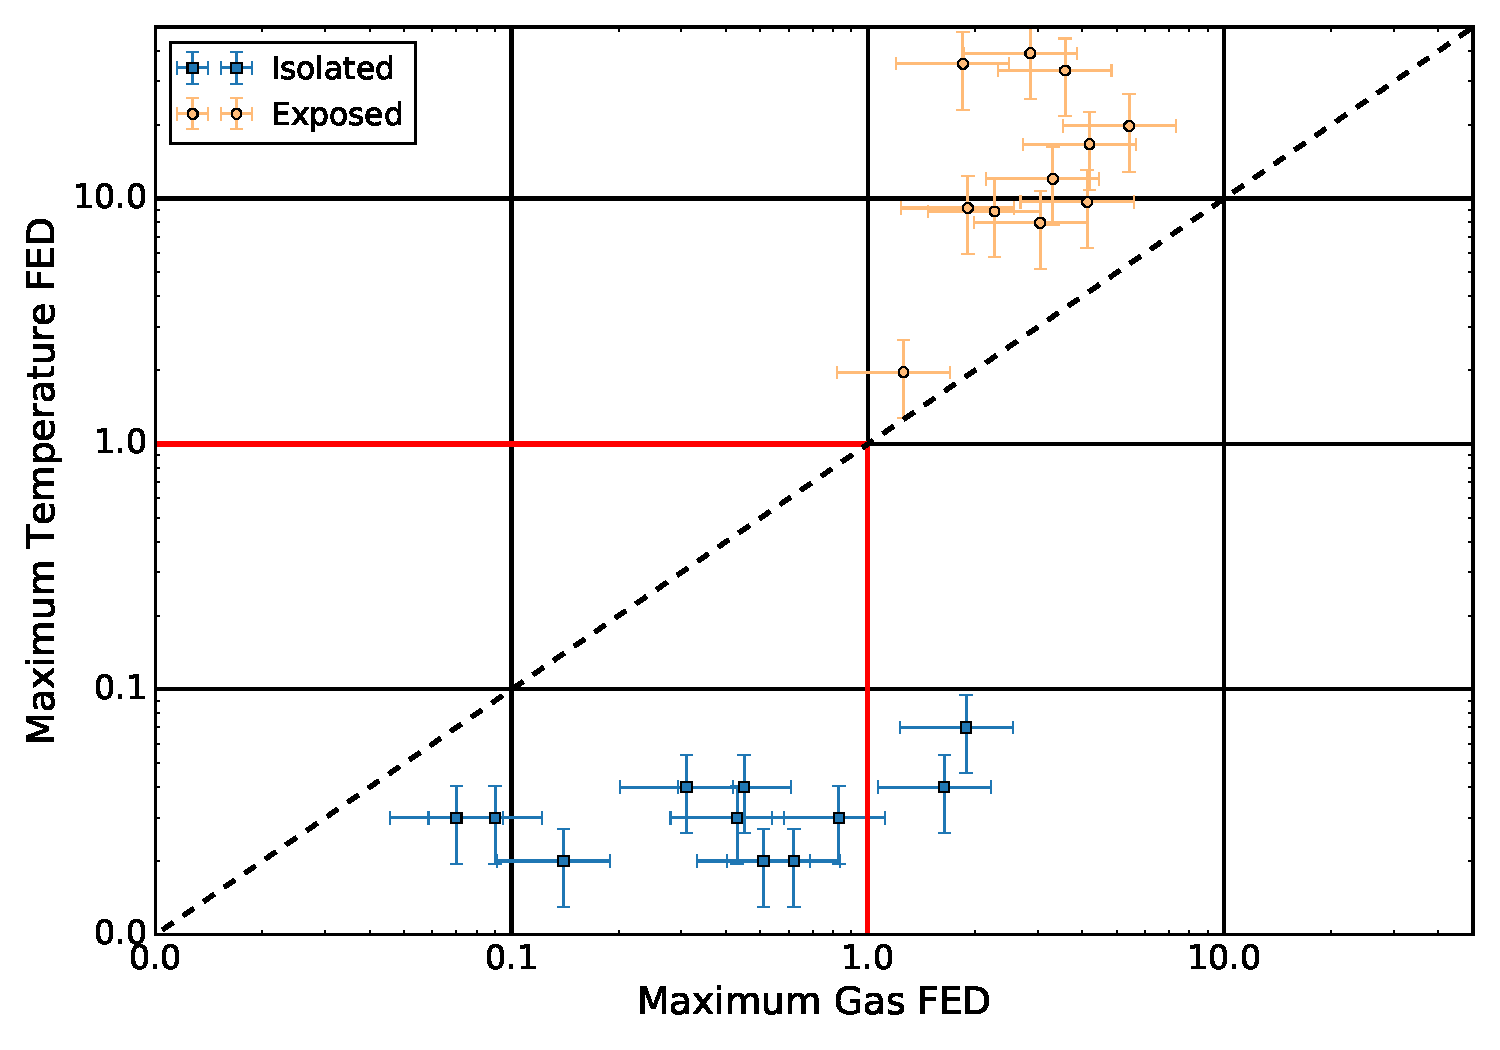
\includegraphics[width=.75\textwidth]{../Figures/br_compare/Near}
	\caption[Maximum Hallway and Near Bedroom FED values]{Maximum Hallway and Near Bedroom FED values. Gas FED is shown on x-axis and Temperature FED is shown on y-axis. Red lines denote the FED at which incapacitation is expected for 50\% of the population is expected (1.0)}
	\label{fig:near_FED_compare}
\end{figure}

The maximum temperature FED in areas remote from the structure and in areas behind closed door was dramatically lower than in the hallway outside of the fire rooms. In the dining room, the temperature tenability threshold was only exceeded in two experiments. In the closed bedrooms, none of the experiments exceeded a temperature FED of 0.07, far less than the threshold of 1.0, where 50\% of the population would receive second degree burns. In each of these other locations, the gas FED is significantly higher than the temperature FED at the end of the experiment, indicating that the exposure to products of combustion in these locations is a greater threat than the thermal insult. In the open areas of the structure, each of the sensor locations that were considered reached the tenability limit,with the exception of the dining room location in Experiment 4. In the closed bedrooms, on the other hand, the tenability limit was only reached in 2 experiments for both the near and far closed bedrooms. Additionally the FED rates in the open locations were higher than those observed in the closed areas.
\begin{figure}[!ht]
	\centering
	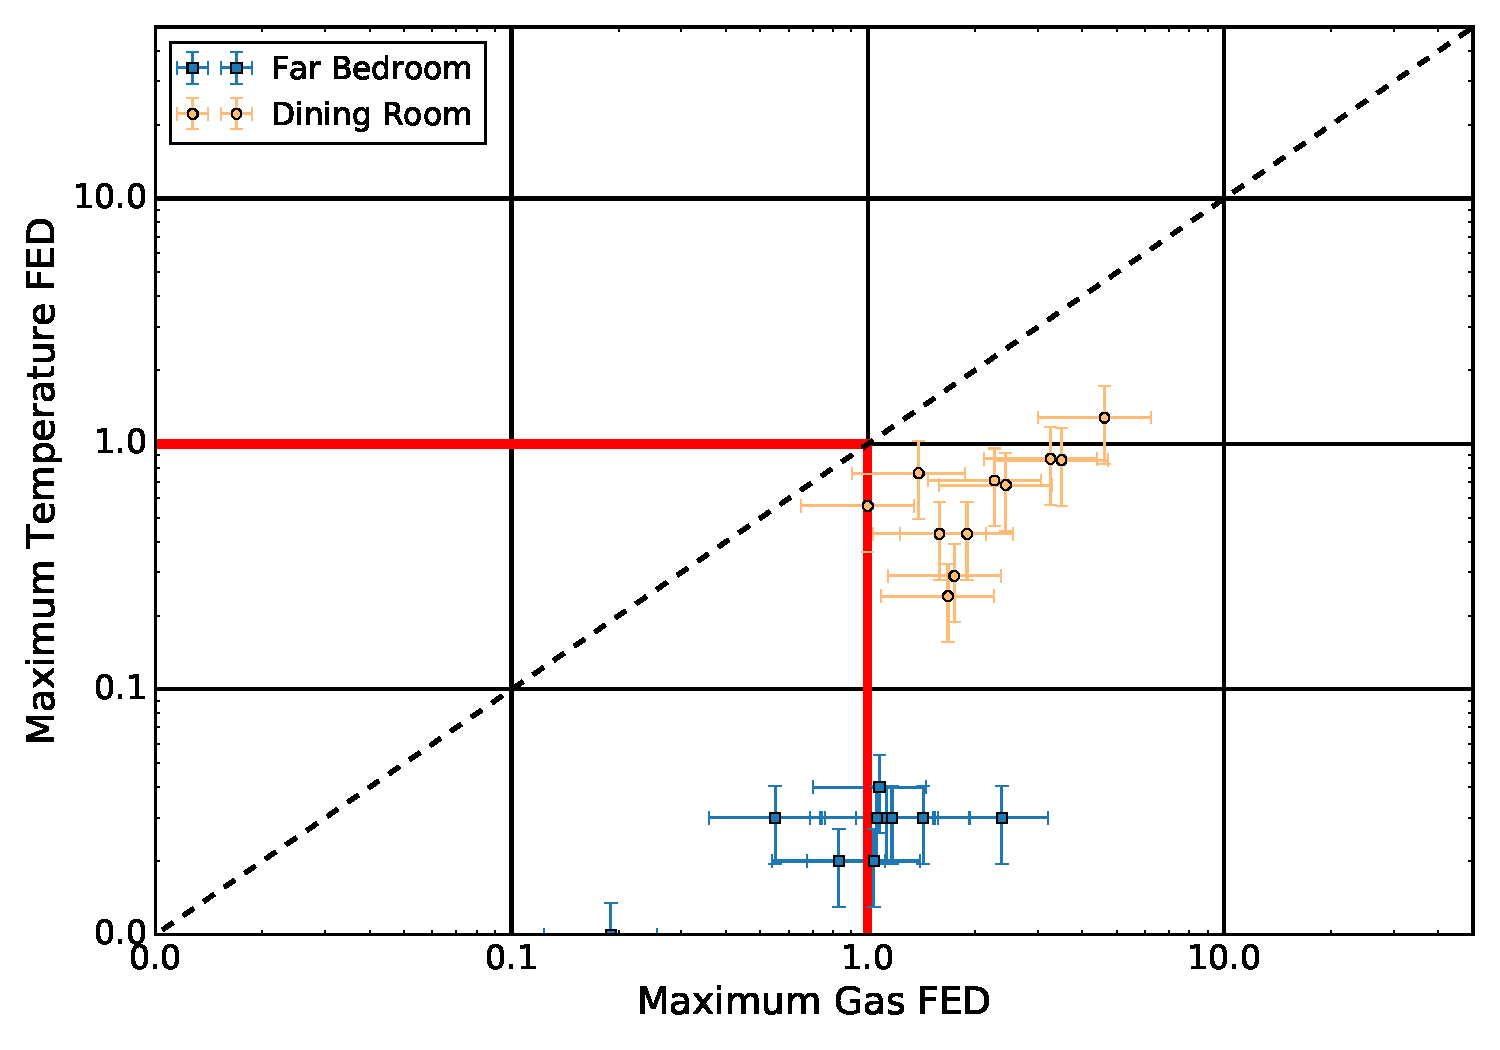
\includegraphics[width=.75\textwidth]{../Figures/br_compare/Far}
	\caption[Maximum Dining Room and Far Bedroom FED values]{Maximum Dining Room and Far Bedroom FED values. Gas FED is shown on x-axis and Temperature FED is shown on y-axis. Red lines denote the FED at which incapacitation is expected for 50\% of the population is expected (1.0)}
	\label{fig:far_FED_compare}
\end{figure}

% These findings are consistent with previous studies [ref], which have identified 

\subsection{Search Methods and Victim Removal}
\label{subsec:search}
The time to find and remove the simulated occupants (victims) in the dining room and the near closed bedroom varied more between the six groups of firefighters that participated in the scenario than between the attack methods, side of the structure, or whether the group had been through the scenario previously. There was no statistically significant difference in the times to locate or remove the victims between the transitional attack method versus the interior attack method. This would indicate that there was not an improvement in visibility as a result of the early water application in the transitional attack scenarios that aided the search crew in finding the victim more rapidly. While temperatures and FED rates dropped following suppression, as described in Section \ref{subsec:ff_int}, the structure was charged with optically dense smoke at the time of entry. While suppression halts the production of products of combustion, the expulsion of products of combustion from the structure is a time-dependent process, and the rate at which smoke is exhausted and visibility is improved is related to the time of suppression and the number and area of ventilation openings.

Once the victims were found by the search team, several different methods were used to remove them from the structure, although two methods were most common: a ``standing drag''[reference fundamentals] and an extremity carry. In the standing drag, one firefighter grabbed the victim beneath their shoulders and either removed the occupant themselves or were assisted by their partner, who grabbed the feet. In the extremity carry, one partner grabbed the simulated victim's wrists while the other grabbed their ankles. Each of these two methods involved the search crew standing upright in order to remove the victim. While standing upright may allow for more efficient movement, and can result in more rapid removal of the victim, it also can result in the victim's head being held higher above the ground than if they were being dragged. Since products of combustion are at a higher temperature, and therefore less dense, than the surrounding gases, it is possible that holding the victim's head higher may expose the victim to higher concentrations of toxic gases. Furthermore, in each of the experiments, victim removal was occurring while suppression was already underway, and water was being applied directly to the fire rooms. Prior to the temperature decreases in the structure following suppression, described in Section \ref{subsec:ff_int}, the 1.5 m (5 ft) temperatures in the hallway and dining room were 577$^{\circ}$C and 216$^{\circ}$C, respectively. These 1.5 m (5 ft.) temperatures are 233$^{\circ}$C and 74$^{\circ}$C higher, respectively, than the corresponding 0.9 m (3 ft.) temperatures. Particularly in areas close to the seat of the fire, the temperatures at the standing height of a firefighter may exceed those where the victim could be removed using a standing drag. Although this series of experiments did not consider searches that occur ahead of the attack team or in severe thermal conditions, it is important to note that these searches may occur, and in such cases where temperatures have not reduced following suppression, potential victims may have to be removed at crawling height, which has the potential to be less efficient, and thus require more time to remove a trapped occupant.  

Conventional firefighting tactics [mittendorf,norman] dictate that areas close to the suspected seat of the fire should be searched first, as occupants trapped in these areas are exposed to the greatest risk. The data from these experiments showed that simulated occupants trapped in open areas close to the fire, such as the near hallway, are indeed at the greatest risk of thermal exposure, but these areas are also the least likely location to find a tenable victim. The highest temperature and gas FEDs were observed in the near hallway. The other victim locations experienced significantly lower FEDs, especially at the time of intervention. Consider Figure \ref{fig:open_FED_compare}, which shows the FEDs at the dining room and hallway at the time that the first victim was found. These locations are approximately equidistant from the front door, and can be compare if the search team first went towards the fire and found a victim, versus if they went away from a fire and found a victim in the same amount of time. The chart shows that the victim that the team who searched away from the fire is more likely to be viable than the victim where the search team searched towards the fire. The same could be said about an occupant trapped in either of the closed bedrooms, where the FED values were negligible at that time.  

\begin{figure}[!ht]
	\centering
	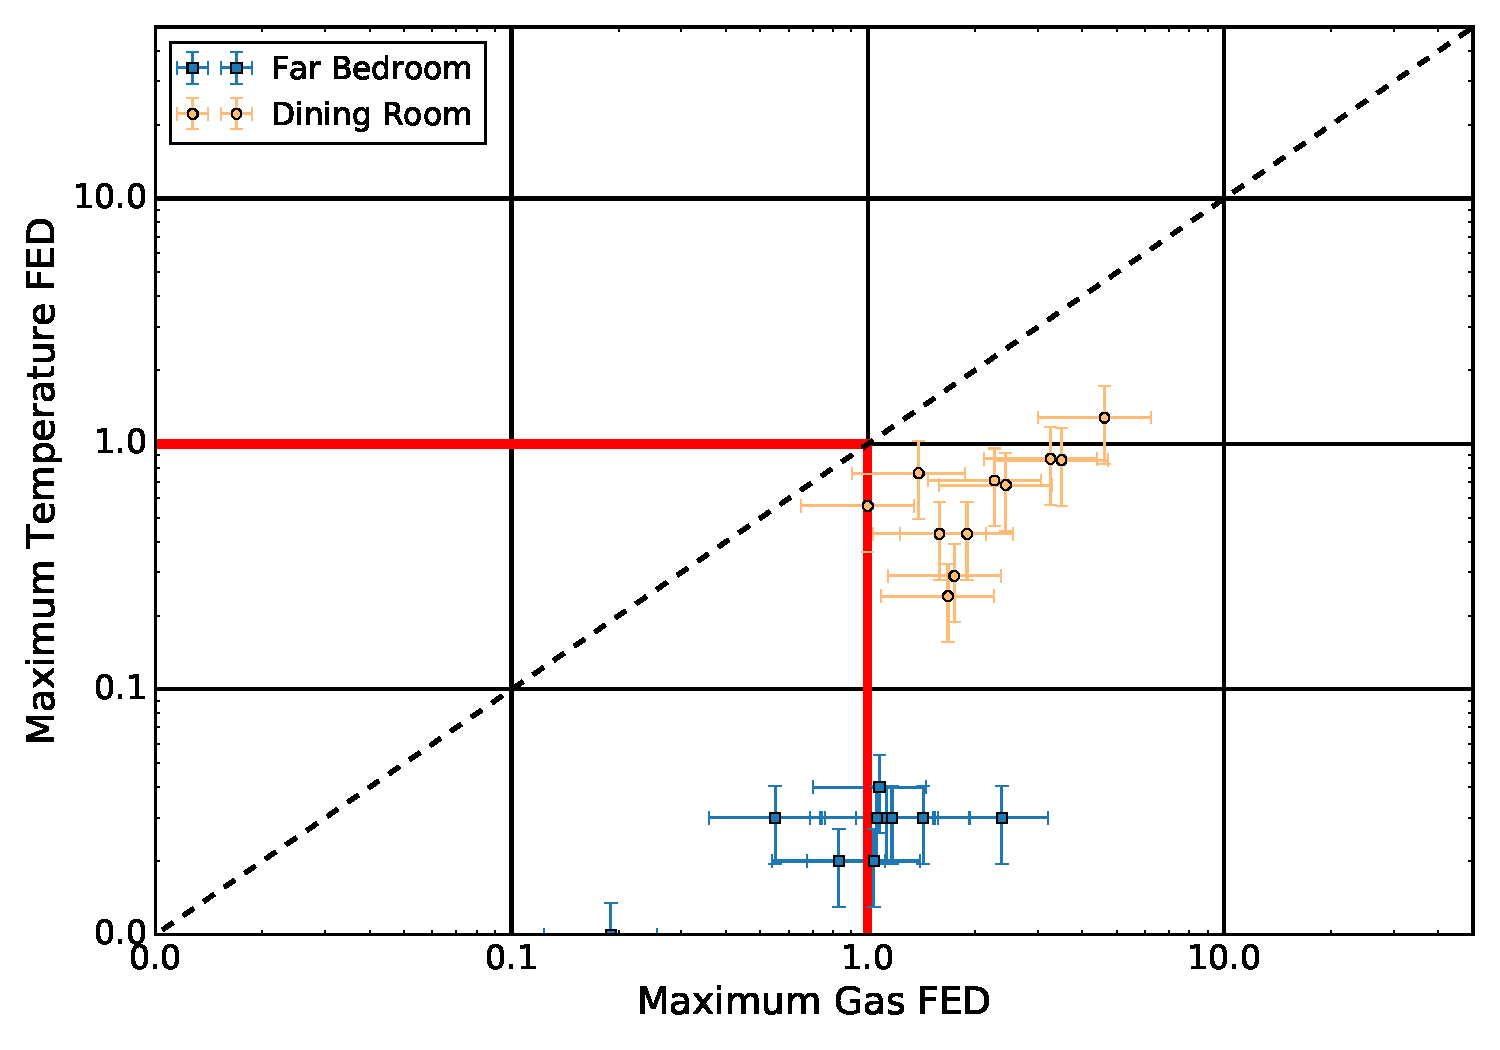
\includegraphics[width=.75\textwidth]{../Figures/br_compare/Far}
	\caption[Near Hallway vs. Dining Room FED values at time of intervention]{Near Hallway vs. Dining Room FED values at time of intervention. Gas FED is shown on x-axis and Temperature FED is shown on y-axis. Red lines denote the FED at which incapacitation is expected for 50\% of the population is expected (1.0)}
	\label{fig:open_FED_compare}
\end{figure}

When considering the times that it took the crews to find and remove victims, it is important to note that the searches in these experiments were conducted in a single-story structure with a relatively simple geometry. Victims were only required to be moved about 6 m (20 ft.) to be extracted from the structure. If the floor plan were larger or more complicated, the times required to find and remove victims may have been longer. Following suppression, the rate of gas concentration decrease was not as high as the rate of temperature decline described in Section \ref{subsec:ff_int}. Thus, although the FED rate was decreasing in the time that the search crew took to find and remove the victims, they were still exposed to high concentrations of toxic gases. Because of the nature of the governing equations, the FED of any trapped occupants would continue to increase until they are removed from the structure. This is demonstrated in Figure \ref{fig:vic_removal}, which plots the increase in FED toxicity from the time that the search crew made entry to the time that the dining room victim is removed. The removal times for all 12 search crew repetitions were considered for all 12 experiments. Note that because there were no local gas concentration measurements for the simulated occupants, the stationary sample point in the dining room was assumed to represent the toxic exposure to the occupant for the duration of the removal process. While it is likely that the gas concentrations and resultant FED exposures would be different within the victim removal path, the dining room concentrations offers an approximation to the toxic insult to the trapped occupant. The chart shows that as the removal time for the simulated occupant increases, the tenability of the occupant is affected dramatically. This emphasizes the importance of rapid removal of victims located during the search in an effort to minimize the toxic exposure of these occupants. 
\begin{figure}[!ht]
	\centering
	\includegraphics[width=.75\textwidth]{../Figures/victim_removal/V1}
	\caption[Relationship between occupant removal time and increase in FED between entry of search team and removal of dining room victim]{Relationship between occupant removal time and increase in FED between entry of search team and remvoal of dining room victim}
	\label{fig:vic_removal}
\end{figure}

In this series of experiments, most of the simulated occupants were removed from the structure out the front door from the location that they were found. The shortest occupant removal time, however, was observed in Experiment 4, where the search crew removed the victim out of the rear door of the near closed bedroom. This removal method exposed the victim to toxic gases for the shortest duration, but also avoided dragging the victim through the hallway and living room, where the  concentrations of products of combustion were higher than in the closed bedroom. Thus, depending on the conditions within the structure, the location of the occupant within the structure, and the knowledge of the search company of alternative means of egress, the ideal path for victim removal may be out of an opening separate from the one which the search team entered through, such as a rear or side door, or even through a window or down a ladder. this emphasizes the importance of situational awareness among the members of the search company and coordination of victim removal. 

\subsection{Attack Methods and Outliers}
\label{subsec:fire_attack}

With the exception of Experiment 3, the attack teams in the transitional attack scenarios applied at least 9 second of water through the window of each fire room. In the majority of these experiments, the water application resulted in a temperature reduction throughout the structure, but most drastically in the fire rooms. The attack crew in Experiment 3 directed their hose steam through the window for a shorter duration than the rest of the experiments, 4 seconds into Bedroom A and 3 seconds into Bedroom B. This short water application, combined with a delay in entry while the search crew forced entry into the structure, allowed for a significant period of regrowth before the attack team reached the hallway to complete final extinguishment. The initial temperature decreases at the 0.9 m (3 ft.) level in each of the fire rooms and the subsequent increases due to regrowth prior to final suppression are listed in Table \ref{tab:exp_3_temps}. Following suppression, the 0.9 m (3 ft.) temperatures decreased by 463$^{\circ}$C in Bedroom A and by 235$^{\circ}$C in Bedroom B. Because of the delay between the short initial attack and the final suppression when the attack team reached the hallway, the 0.9 m (3 ft.) temperatures increased 269$^{\circ}$C and 567$^{\circ}$C in Bedrooms A and B, respectively. The temperatures in Bedroom B at the that the attack team reached the end of the hallway were consistent with a postflashover compartment fire. If the delay between initial and final suppression were longer, it is likely that conditions remote from the fire room would have started to deteriorate. The regrowth following the exterior attack in this experiments resulted in a longer gap between suppression and the time at which the FED rate began to decrease. Thus, by failing to apply a sufficient amount of water  during transitional attack, the effectiveness of the attack in improving conditions within the structure is limited. 

\begin{table}[!ht]
    \centering
    \caption{Temperature Reduction and Subsequent Regrowth in Experiment 3}
    \label{tab:exp_3_temps}
    \begin{tabular}{ccc}
    \toprule[1.5pt]
 	 Event 																	&	Bedroom A 0.9 m (3 ft.) &	Bedroom B 0.9 m (3 ft.) \\
 	\midrule 
  	Temp. ($^{\circ}$C) prior to exterior suppression 						&	585						&	820						\\
  	Minimum temp. ($^{\circ}$C) following exterior suppression				&	154						&	585						\\
  	Maximum temp. ($^{\circ}$C) prior to final,								&	423						&	1152					\\
  	 interior suppression													&							&							\\
 	\bottomrule[1.25pt] 
    \end{tabular}
\end{table}

Just as the duration of water application is important to the effectiveness of the attack, the location to which the water is applied is important. In the transitional attacks, the exterior water application occurred directly into the two fires rooms, resulting in a drastic reduction in temperatures when a sufficient amount of water was used. In the interior attacks, several groups applied water between the time they entered the front door and the time they reached the hallway. The poor visibility within the structure during this time makes it difficult to assess the effectiveness of these initial bursts of water, but the most effective cooling in the interior attack experiments occurred once the attack crews had reached the hallway, allowing them to apply water directly to the contents of the burning rooms. In one experiment, Experiment 5, the attack crew did not apply any water until reaching the hallway. Upon reaching the hallway, an issue was encountered with the hose advancement, and the nozzle firefighter opened the nozzle, but was only able to apply water to the ceiling of the hallway. The hose advancement issue was thereafter resolved, and the nozzle firefighter was once again able to advance and complete extinguishment. Prior to this final extinguishment, the temperature decreases in the area of the fire room were negligible, indicating that the water application was ineffective. The results of this scenario indicated that it is important that in order for effective  and definitive suppression, water must applied directly to burning fuels.

The suppression methods employed in this series of experiments indicated that, in order for suppression to be effective in improving conditions within the structure, a sufficient quantity of water must be applied to the burning contents of the room. In the transitional attack, water was applied earlier in the experimental timeline, resulting in a reduction in temperatures sooner than when compared to the interior attack experiments. After deploying their attack line, the crews conducting transitional attacks were able to immediately apply water to the fire, resulting in water application significantly faster than the interior attack groups and a reduction in temperatures sooner than when compared to the interior attack experiments. Once the interior attack groups deployed their hose line, they were often delayed while waiting for the search crew to simulate forcing entry into the building. Despite the delay, the interior attack groups entered the structure significantly faster (174$\pm$10 s) when compared to the transitional attack groups (213$\pm$29 s) (p=0.02). Despite the early water application in the transitional attack experiments, there was no significant difference in the time at which the FED rate began to decrease between the two attack methods. 

\subsection{Limitations}
 The equations used to compute the FEDs at each of the sample points for these experiment have a great deal of uncertainty associated with them, as high as 35\% in some cases. This high uncertainty, combined with the uncertainty of the measurements themselves, resulted in a large amount of scatter in the gas concentration data. Additionally, significant gas concentrations were measured until the gas layer had descended to the point of the sample location, which in some experiments occurred later than others. The large variation in gas concentrations was not noted in the temperature measurements, indicating that although the thermal conditions within the structures were within a reasonable margin of uncertainty, the gas concentrations may be more susceptible to scatter. The gas sample locations in this series of experiments were fixed, which made accounting for the toxic exposure to victims during their removal from the structure difficult. Future work should attempt to assess how the victim's toxic exposure changes during the removal process. 

\section{Conclusions}

12 full scale fire experiments were conducted in a 111 m$^2$ structure constructed to be representative of a single family dwelling constructed in the late 20th century. The structure was instrumented with temperature measurements in each room and gas concentration measurements in the hallway between the two fire rooms; the two uninvolved, closed bedrooms; and the dining room. Two 61 kg (135 lb.) firefighter training mannequins were placed in the dining room and the closed bedroom closest to the fire rooms in order to simulate occupants who were trapped within the structure. 6 groups of firefighters, recruited from fire departments throughout the country, participated in two experiments each. Each group included an attack team and a search team, each of which consisted of two firefighters. The attack team executed either a transitional attack or an interior attack, and the search team searched for the simulated trapped occupants in a pattern starting away from the fire. 

The results showed that there was a large variation in the times it took the 6 groups to complete various fireground tasks. The standard deviation of the groups' times to execute various fireground actions ranged from 20\% to 95\% of the average times. This emphasized the importance of training to develop proficiency in tasks such as hose advancement, forcible entry, and search techniques, as well as coordination between companies on the fireground to minimize miscommunication and improve efficiency. The variation in temperatures at the 0.9 m (3 ft.) height at the time of firefighter intervention were within an acceptable margin of the combined uncertainty of the instruments, while the variation in gas concentrations was considerably higher. 

Gas concentration and temperature measurements were analyzed using a fractional effective dose (FED) approach. The results indicated that a closed bedroom door was effective at isolating the contents of the room from toxic products of combustion. The FEDs within the two closed bedrooms were found to be significantly lower than locations just outside of the closed door. Occupants trapped in the closed bedrooms would likely have been tenable well into the experiment. The most severe toxic and thermal exposures that were measured were in the hallway outside of the two fire rooms. This was the only location within the structure where incapacitation due to thermal insult occurred prior to incapacitation due to toxic gas exposure. This is consistent with fire victim data where occupants found close to the  origin of the fire typically sustain severe thermal injuries, but have relatively low carboxyhemoglobin levels. The thermal exposure in other areas of the structure decreased as distance from the fire room increased, particularly in isolated areas. 

Water application by the fire attack teams was associated with a rapid drop in temperatures throughout the structure, followed shortly afterward by a decrease in the FED rate. There was no significant difference between the magnitude of the temperature decrease or the time until the inflection point in the FED curve between transitional attack and interior attack. For the transitional attack scenarios, water was applied to the fire significantly earlier in the experimental timeline than in the interior attack scenarios, while in the interior attack scenarios, the attack team made entry to the structure significantly sooner than in the interior attack scenarios. In one of the transitional attack experiments, the exterior water application was not sustained for a sufficient amount of time, allowing for regrowth of the fire, resulting in temperature rebound in areas close to the seat of the fire and a substantially longer time until the FED rate began to decrease. Similarly, for the interior attack scenarios, significant improvements within the structure were not noted until the attack team was able to direct water directly onto the burning contents in the bedrooms. For both attack methods, significant improvements in  interior conditions were observed following effective water application, while ineffective water application reduced or delayed the positive effects.

The time from search team entry to removal of the dining room victim ranged from 20 seconds to 158 seconds. During this time, the simulated occupant would have been exposed to toxic products of combustion. As the removal time for the victim increased, the toxic exposure to the victim increased, despite the decreasing FED rate due to suppression. This observation is consistent with the nature of the FED method, as the FED will always increase until concentrations return to ambient. The search crews in these experiments were directed to search in a pattern away from the fire, although some fire service literature dictates that the search should begin close to the seat of the fire to find the victims that are most threatened. In these experiments, a victim located at the hallway would indeed have been more threatened at the time that the search crew reached and located them, but the victim would also have been less likely to be tenable compared to the same victim located in the dining room. The victim tenability analysis highlighted the guidance in fire service literature, that the search should attempt to focus on the victims that are most threatened, although showed that threatened victims are not always closest to the seat of the fire. Additionally, the results emphasized the need for rapid removal of occupants to limit toxic exposures. The results of the 12 experiments conducted indicated that a successful fire attack in terms of maximizing the probability of occupant tenability involves the coordination of suppression tactics to promptly and effectively deliver water to the fire and reduce the thermal and toxic insult to potential occupants with rapid identification and removal of the occupants. 



\end{document}